
\section{System}\label{sec:System}
\todo[inline, color=red]{Laura}
The actual application can be divided into two types of VR rooms. First of all there is a learning room (compare section~\ref{sec:Learningroom}), where the user can get in touch with the different interaction methods and afterwards different tasks will be presented to him in a VR supermarket scenario (compare section~\ref{sec:supermarket}). \textcolor{red}{@Laura: Evtl aus dem letzten Satz zwei sätze machen? etwas verschachtelt und ich hab den gegenpart zu 'first' erst noch gesucht ;)} In the learning room the user will be supported in his learning process by a selfteaching system (compare section~\ref{sec:selfteaching}), which he can switch on and off, when he is in the supermarket. The user can make this setting among all other settings in a Menu  (compare section~\ref{sec:Menu}), which is controllable with the \textit{HTC Vive}-controller. In this menu he can also choose between all provided interaction methods, which are described in section~\ref{sec:Interactions}.

\subsection{VR Labor}\label{sec:VRLabor}
%\todo[inline, color=yellow]{Anna}
In this section the different rooms of the VR Labor will be described. Each room is realised as a \textit{Unity} scene.\\
There are two different kinds of rooms. First there is a simple room to get familiar with the system and the methods, which were implemented. This room will be specified in  section \ref{sec:Learningroom}.\\
The second room is created to look like a small supermarket, in which the user has to solve different tasks (compare section~\ref{sec:tasks}). This room will be described in section \ref{sec:supermarket}.

\subsubsection{Learning room} \label{sec:Learningroom}
The learning room is the first room where the user will get to know the system. On one hand the user will get familiar with the virtual experience and the \textit{HTC Vive} system (HMD and controller) and on the other hand the user will learn the different interaction methods. 

\begin{figure}[H] 
	\center 
	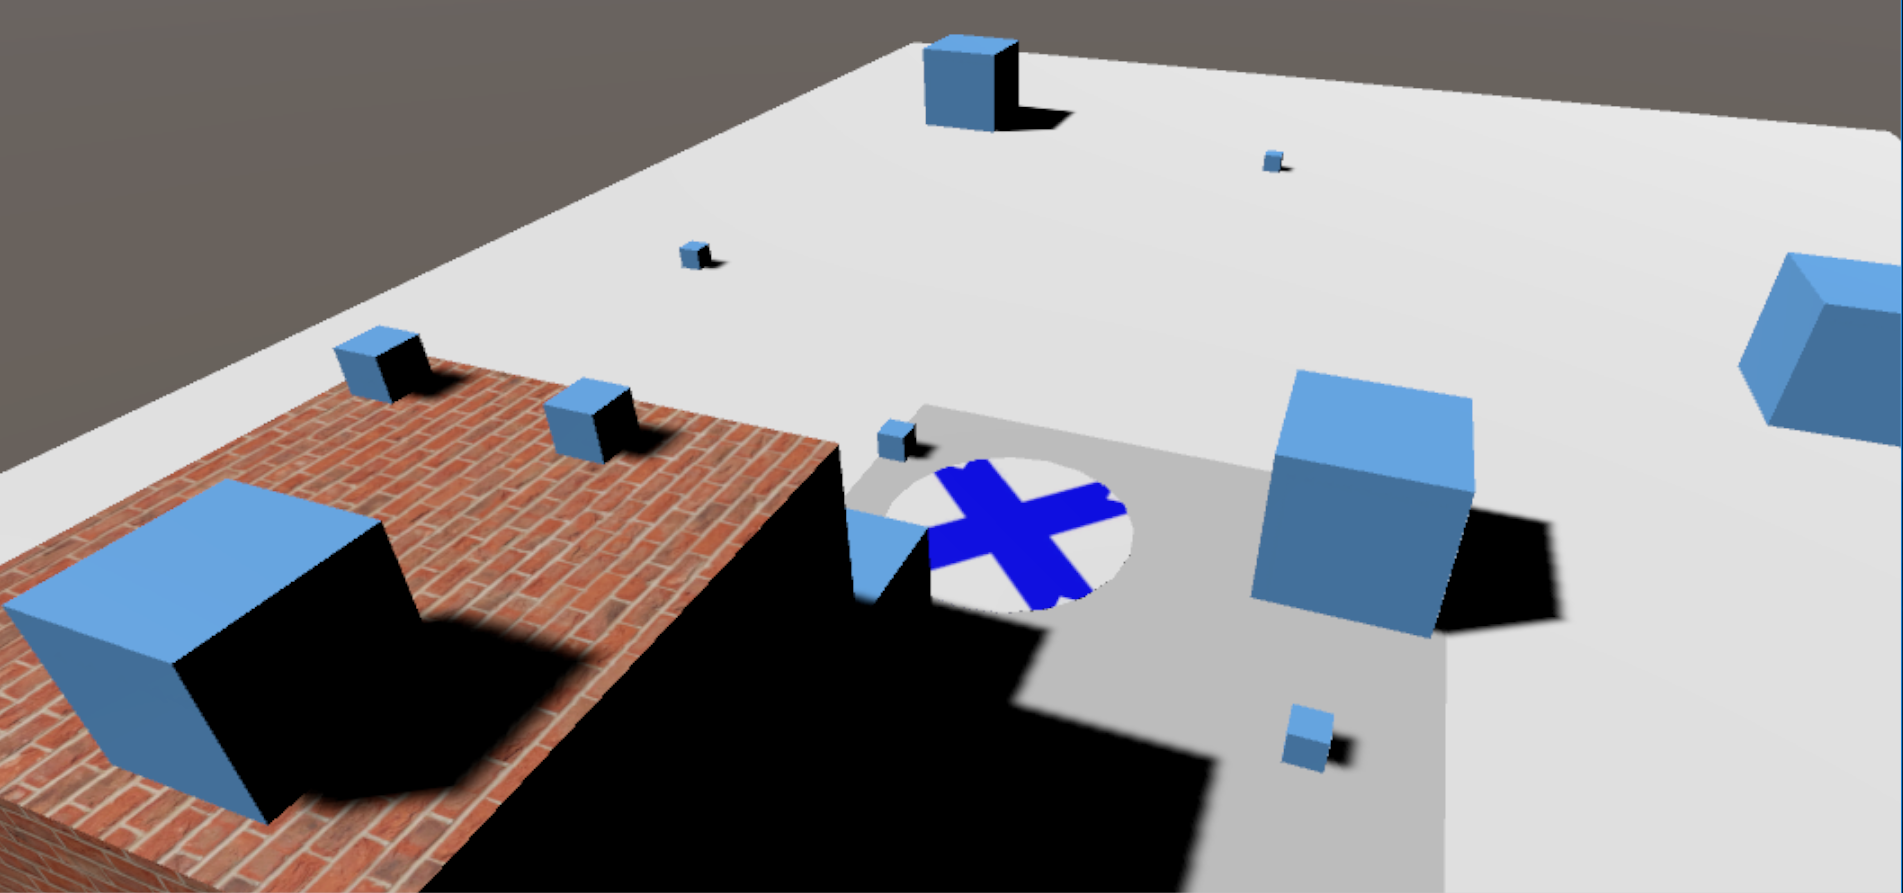
\includegraphics[width=12cm]{Images/learningRoom2.PNG}			
	\caption[Overview of the Learning Room.]{Overview of the Learning Room.}
	\label{fig:learning room}
\end{figure}

The room is designed very clean and simple. In different sizes and distances simple objects, in this case cubes, are distributed randomly. This is shown in figure \ref{fig:learning room}. The virtual room is slightly bigger than the usable room in reality. So the user is forced to user interactions, which are designed for larger distances, to move some objects (compare sections~\ref{sec:Raycast} and~\ref{sec:ExtendableRay}). Due to different colors of the floor the user know how big the real room is approximately. In addition the \textit{HTC Vive} system offers a coloured wire, which is shown in the HMD, whenever the user gets too close to the border of the calibrated area.\\
The user should already know the different interactions as well as the menu settings, when he enters the supermarket scene. So the menu and interactions are similar in both rooms. Also the labelling of the target object and the reaction of the target area to the target object will be established. This will be described in section~{sec:tasks}.\\ 
To get to know all settings and methods the user will be led to the entire learning room by a selfteaching system. This selfteaching is be described in section \ref{sec:selfteaching}. 


\subsubsection{Supermarket} \label{sec:supermarket} 
The second room is a small supermarket. 

\begin{figure}[H] 
	\center 
	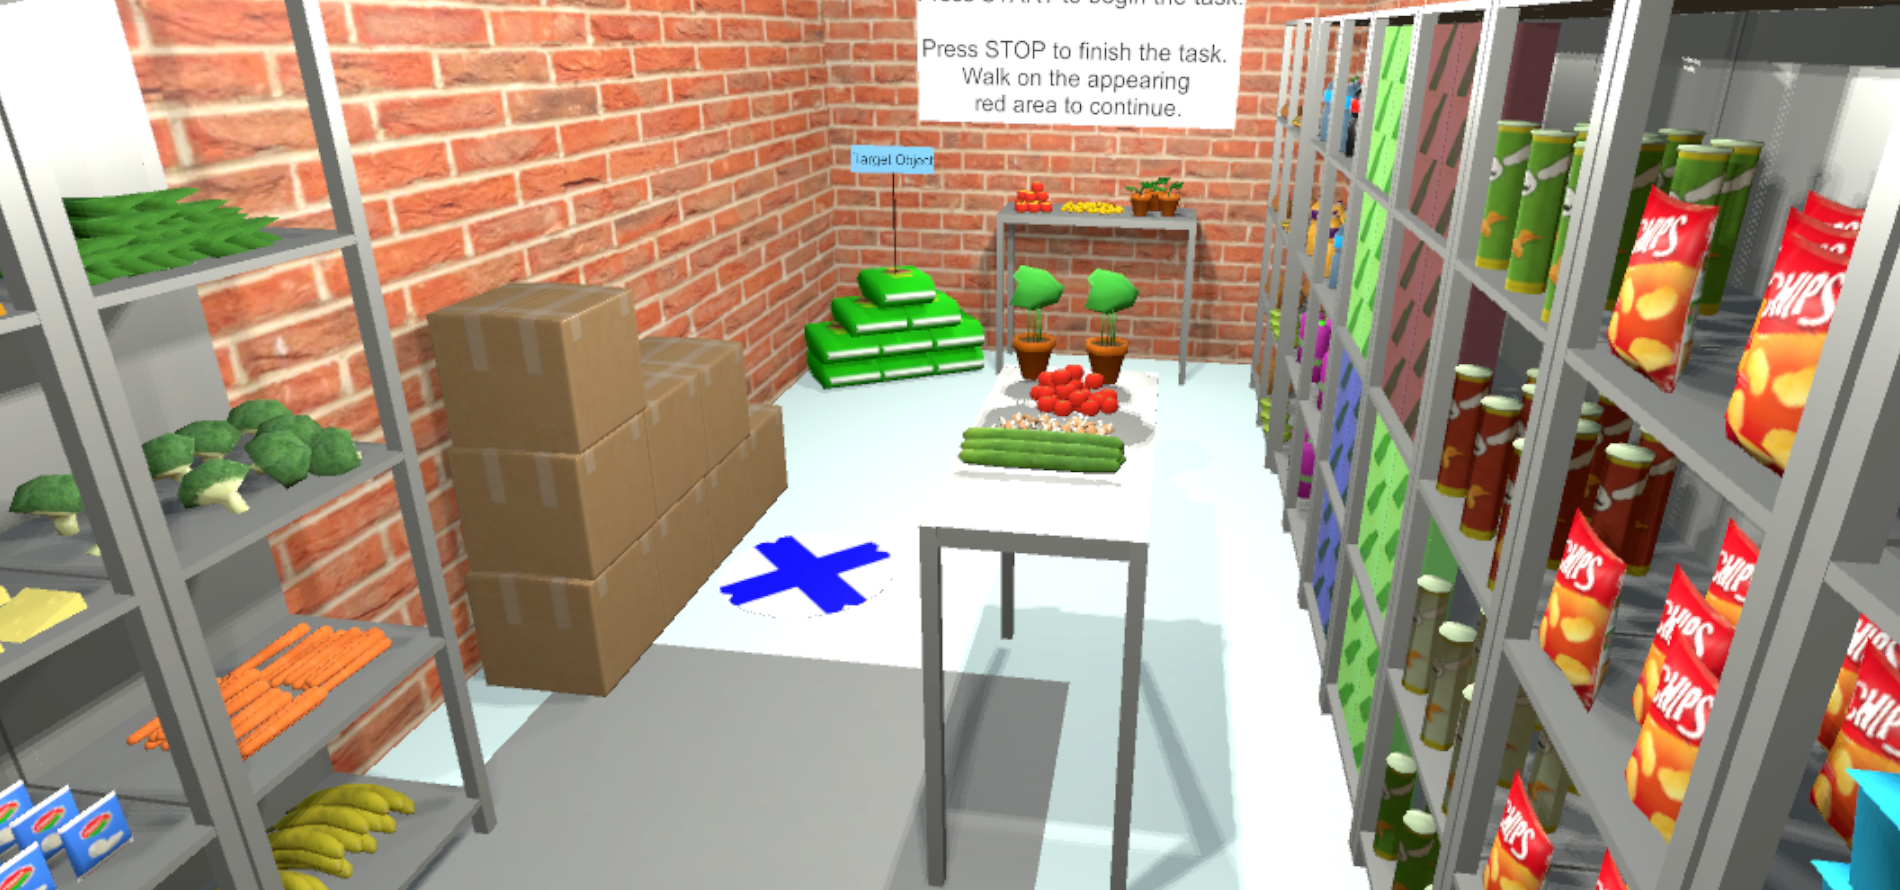
\includegraphics[width=12cm]{Images/supermarket.PNG}
	\caption[Overview of the supermarket.]{Overview of the supermarket.}
	\label{fig:supermarket}
\end{figure}

Like it is shown in figure \ref{fig:supermarket} in this supermarket are different sized objects in various distances. All objects could be found in a real supermarket, from fruits to milk. This objects were dowloaded from the asset store \cite{asset_food1} \cite{asset_food2} \cite{asset_box}. \\
The size of the real room is also displayed by using a slightly darker colour on the floor of the supermarket. This is necessary, because the supermarket is bigger than the real room. So interactions for far distance have to be used according to the tasks.

\begin{figure}[H] 
	\center 
	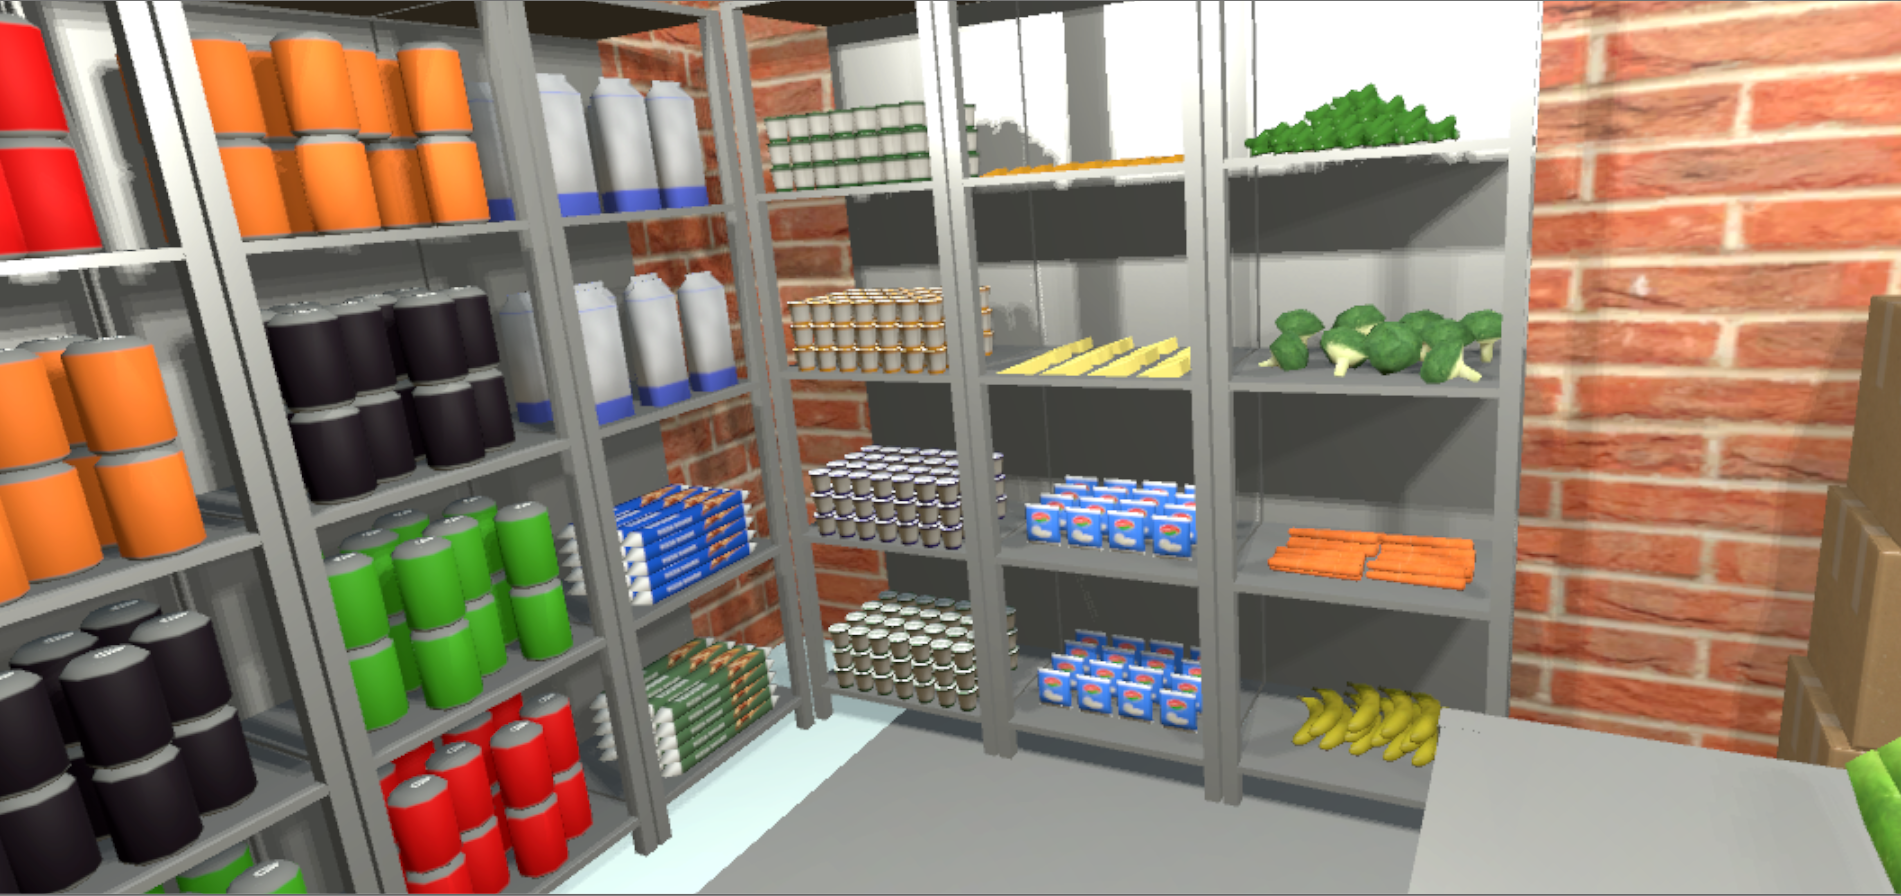
\includegraphics[width=12cm]{Images/supermarket2.PNG}
	\caption[Closer View of the Shelves.]{Closer view of the Shelves.}
	\label{fig:shelve}
\end{figure}

In some tasks the participant has to grab objects which are hard to pick. On one side they could be at a lower position, on the other side they could have to move other objects before they reach the labelled object. To implement this into a supermarket naturally shelves, like in figure \ref{fig:shelve}, are appropriate for a supermarket. This shelves were build with different scaled cubes.

\begin{figure}[H] 
	\center 
	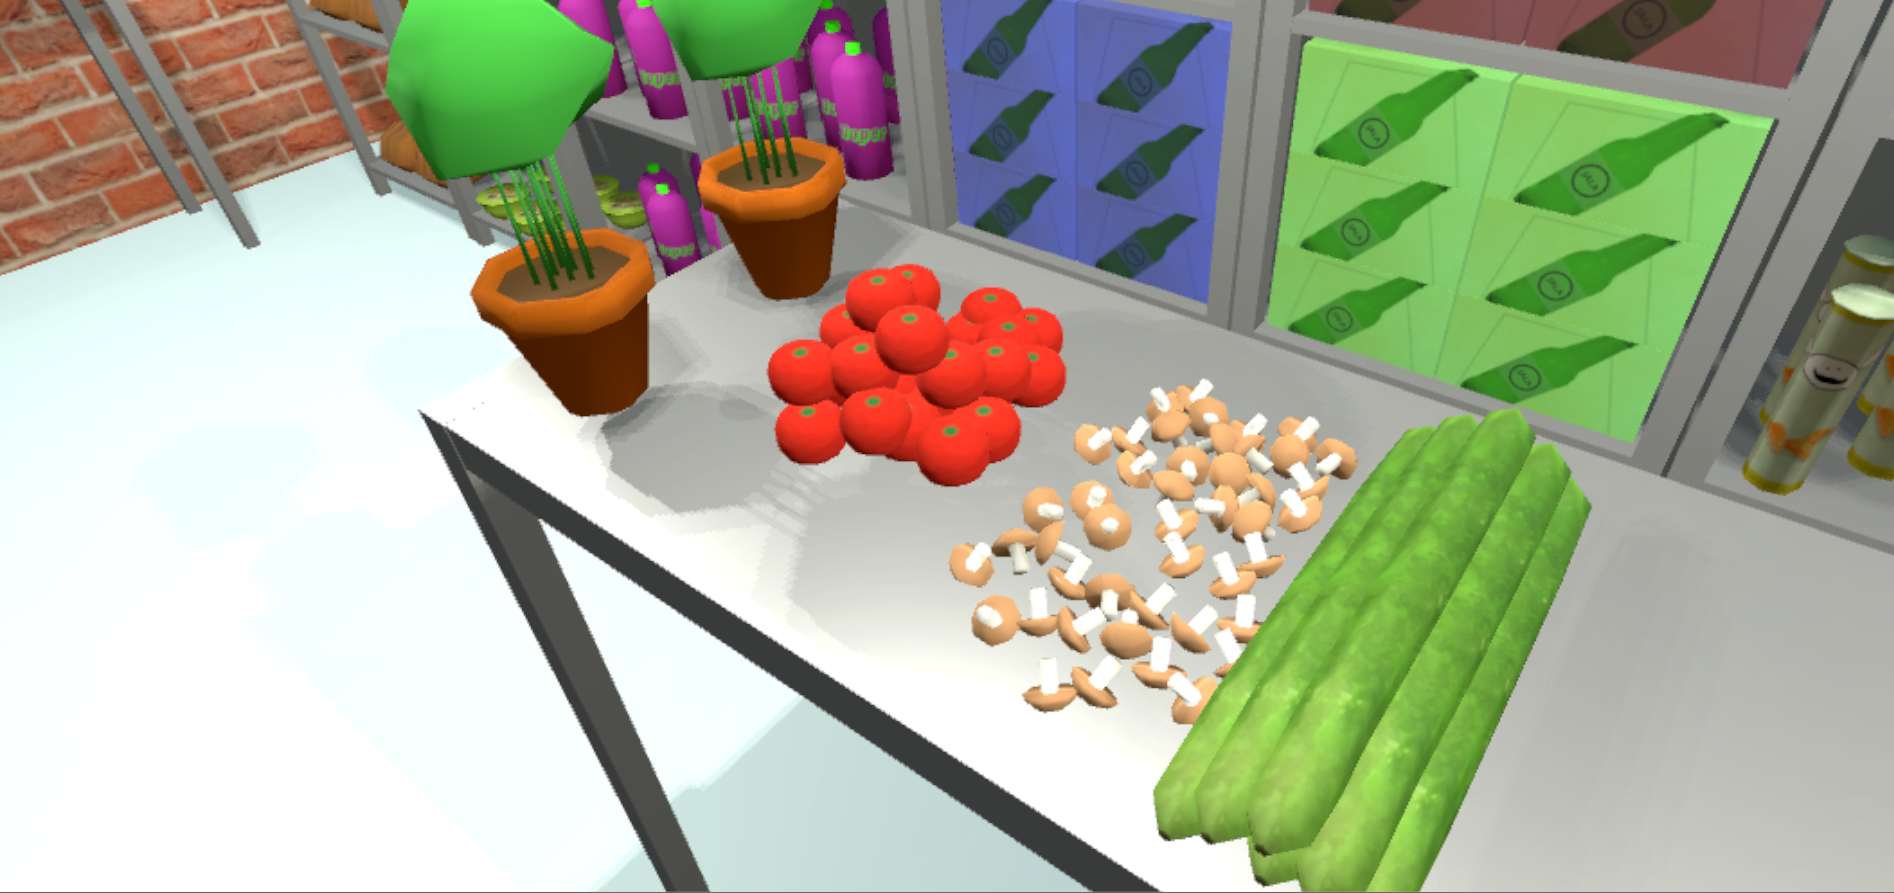
\includegraphics[width=12cm]{Images/supermarket1.PNG}
	\caption[Closer View of the Table.]{Closer View of the Table.}
	\label{fig:table}
\end{figure}	

In a real supermarket objects are not always arranged in shelves. Due to this fact and to have a variance for the tasks,  some objects where placed on tables as one bulk, for example fruits and vegetables. There are two tables in this supermarket. A closer look to one of this tables is given in figure \ref{fig:table}.\\
Depending on the task different target areas can appear in the supermarket. In this situations different objects will be blend out. Also the target object of every tasks will be labelled. The first target area and target object are shown in figure \ref{fig:supermarket}.\\
 The structure of the labelling of the target object are specified in section \ref{sec:selfteaching}.
The different tasks as well as the reaction of the target area to the target object will be described in section \ref{sec:tasks}.

\subsection{Controller Menu} \label{sec:Menu}
\todo[inline, color=red]{Anna}
The controller menu is the main menu of the system. It allows to change settings without leaving the virtual environment. Within this menu interaction methods can be changed and settings like snapping for the interactions can be enabled. In the learning room	the user is able to turn the selfteaching informations on and off. In the same way the user can decide if the tasks will be shown or not in the supermarket. In the supermarket scene the user can restart a single task via the controller menu. With the reset button the scene will be reloaded. The main menu is shown in figure~\ref{fig:mainMenu}.

\begin{figure}[H] 
	\center 
	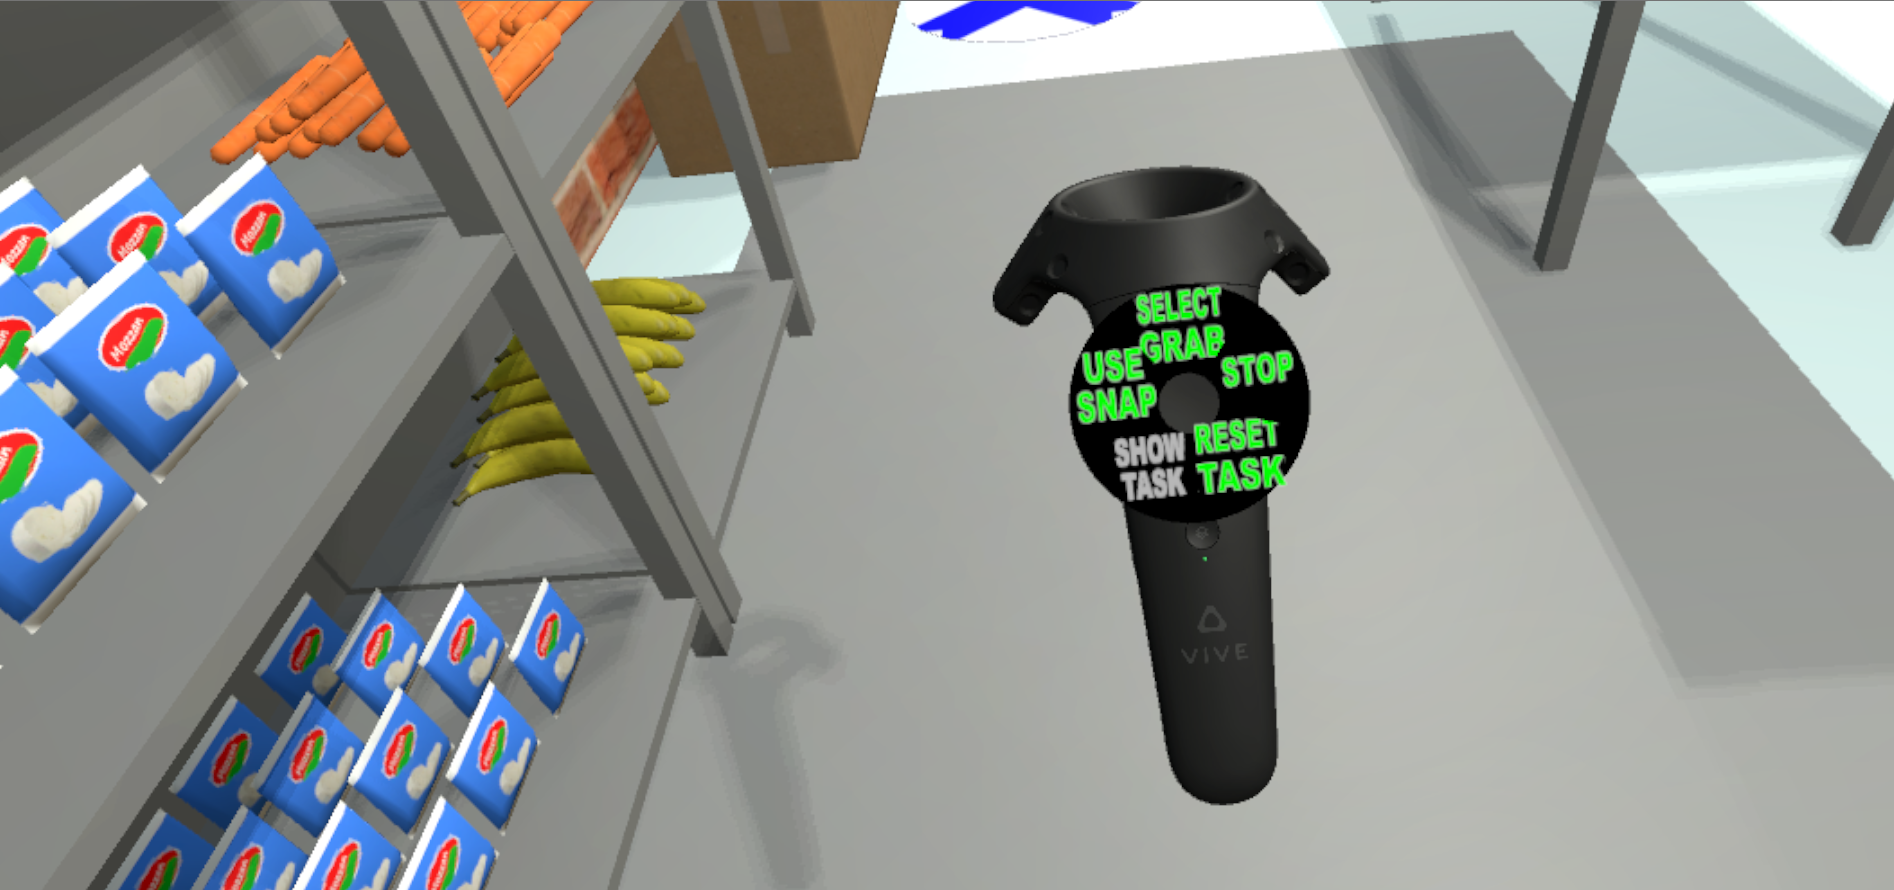
\includegraphics[width=12cm]{Images/Menu1.PNG}
	\caption[Main Menu of the Controller Menu.]{Main Menu of the Controller Menu.}
	\label{fig:mainMenu}
\end{figure}

If the button ``select grab'' is available, the user is able to choose every interaction method he likes. The button leads to an other menu. In this menu the methods are shown as icons, see figure \ref{fig:grabMenu}. The user learns the meaning of those icons with the help of the selfteaching, while they are in the learning room. 

\begin{figure}[H] 
	\center 
	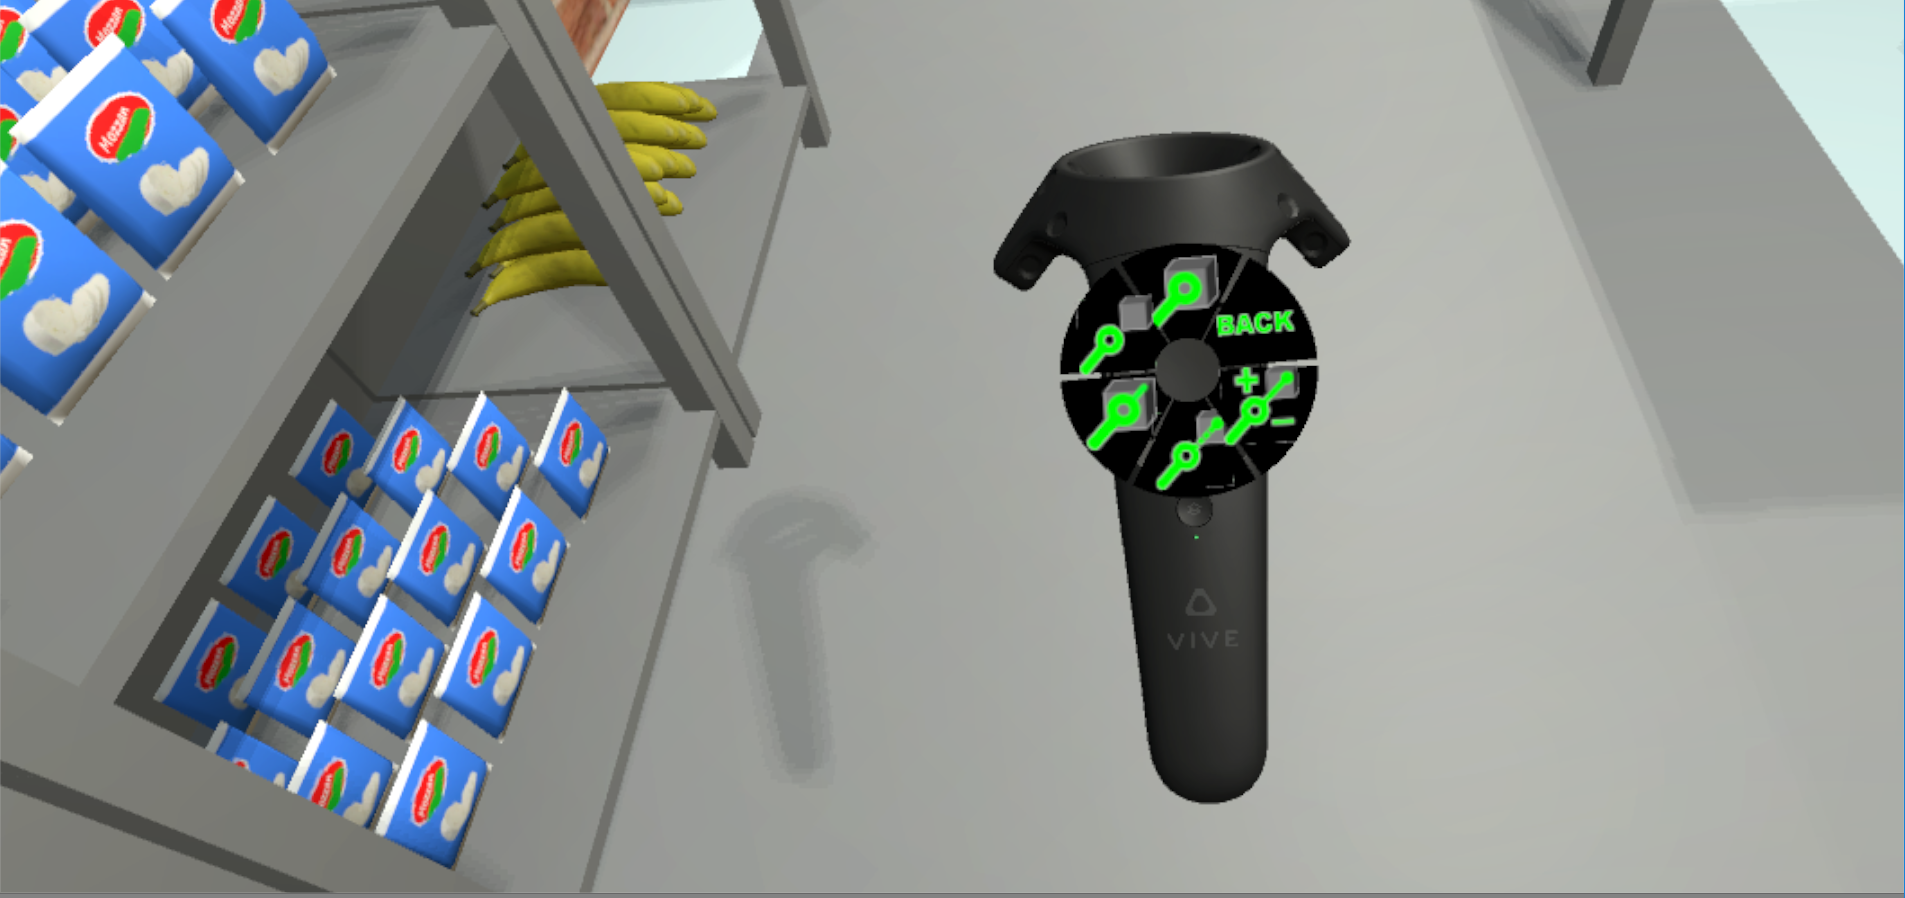
\includegraphics[width=12cm]{Images/Menu2.PNG}
	\caption[Select Grab Menu.]{Select Grab Menu.}
	\label{fig:grabMenu}
\end{figure}

For the measurement, which are described in section \ref{sec:measurement}, the user has to start and stop every tasks. The start button will be the first menu button in every scene. Only if this button is pressed the user can interact with the environment and will be led to the next menu. When the user presses the stop button the switching area will appear and the corresponding \textit{BoxCollider} \cite{website:BoxCollider} will be enabled. If the user reaches this area the next scene will be loaded.\\
The structure of the menu is built on the plug-in ``VRTK'' (Virtual Reality Toolkit) \cite{asset_VRTK} \cite{VRTK}.\\
\textcolor{red}{@Anna: Die VRTK müsstest du schon in den Materialien erklären. Ich denke dann kann man den nächsten Absatz auch ein bisschen kürzer schreiben.}
This is a free packet with different scripts and prefabs for interaction in the virtual reality. From this plug-in the radial menu is used for the controller menu. This creates menu buttons over the touchpad of the \textit{HTC Vive} controller. By scrolling over the touchpad the button can be selected. The selection will be shown by highlighting the button. If this button should be executed, the touchpad has to be pressed when the button is selected. The number of buttons per menu can be changed within the \textit{Unity} editor. Each button can get a different icon. Through a link to a functionof a script this function can be executed if the button is pressed. In this project there is a script named \textit{Menu.cs} in which all functions for the menu are collected. Due to this script different settings can be chosen.


\subsection{Interaction Methods}\label{sec:Interactions}
\todo[inline, color=red]{Laura}
Of course there were various different \textcolor{red}{@Laura: ist das nicht irgendwie doppelt gemoppelt? various und different?} interaction methods required to make the \textit{Interaction Lab} suitable for the testing described and evaluated in section~\ref{sec:evaluation}. Also all interaction methods are implemented to realise the grabbing of virtual objects, they can be separated in the two categories, described in the next two paragraphs:

\paragraph{Close Range (CR) Interactions:} The CR can be interpreted as a synonym for the natural interaction radius of the person. Due to this definition it is excluded that those interactions can be used outside an area, which the person can not reach with his arm, or to be more precise: with the controller in his hand. In other words: the CR combines all interactions which can be used to pick up objects in the direct reach of the user.

\paragraph{Far Range (FR) Interactions:} Due to a limitation of the range of motion in VR applications, it is common to have grabbing interactions, which allow the users to grab objects which \textcolor{red}{@Laura:doppelt which... vllt: interactions designd for grabbing objects which... oder so ähnlich} are normally seen as out of their reach~\cite{VRBook}. Interaction methods allowing such an acting are called FR interactions. It is not excluded, that a FR interaction is used in the actual reach of the user. \\

Whereas the CR interactions differ mainly in the accuracy of the selection of an object while grabbing it, the FR methods differ in their usability. All characteristics of the various interaction methods can be traced in their descriptions (compare sections~\ref{sec:TouchGrab} -~\ref{sec:RaycastHMD}).

For a better understanding it should be mentioned, that all interaction methods can be controlled with the \textit{HTC Vive}-controller. Even there are plenty of different possibilities to grab an object all methods have in common that the grabbing is caused by pressing the trigger on the \textit{HTC Vive}-controller. The releasing of the object is than triggered by letting it go. Whenever there is a divergent usability necessary, it is described in the respective section (compare~\ref{sec:ExtendableRay}).

Due to an easier integration into the learning room (compare section~\ref{sec:Learningroom}), as well as the actual supermarket scenes (compare section~\ref{sec:supermarket}) all methods using a ray (compare sections~\ref{sec:ExtendableRay},~\ref{sec:Raycast} and ~\ref{sec:WandGrab}) are summed up in one script called \textit{AllRaycastMethods.cs}. All other methods have their own script in which the grabbing and releasing is implemented. Also the \textit{Raycast Head Mounted Display}-method, described in section~\ref{sec:RaycastHMD}, is using a ray it is not included into the script mentioned above. This is caused by remaining problems during the implementation of this method which lead to an unfinished work. Further explanations on why this method is not available in the \textit{Interaction Lab} can be found in the according section.

The two interaction methods, described in sections~\ref{sec:TouchGrab} or rather~\ref{sec:ProximityGrab}, can be used with snapping or without it. This technique is used to reassign the position and orientation of a grabbed object in hand. By assuming that the middle of the ring of the \textit{HTC Vive}-controller is the new center of the grabbed object the actual grab could appear more realistic to the user. 

In the application all objects, which can be grabbed are tagged as moveable.\\

In the following sections all available interaction methods of the \textit{Interaction Lab} are presented. To guarantee a better overview they are sorted by their interaction range. 

\subsubsection{Close Range: Touch Grab} \label{sec:TouchGrab}
\todo[inline, color=red]{Laura}
When the \textit{Touch Grab} interaction method is selected the user can make use of the \textit{HTC Vive}-controller to pick up objects directly by touching them and pulling the trigger. To release the object the trigger needs to be released as well.\textcolor{red}{@Laura: Hast du oben nicht geschrieben, dass das eh für alle gilt?} An object can be grabbed whenever it is tagged as moveable and collides with the \textit{HTC Vive}-controller. This collision is detected by giving the object a collider, which fits its form best \cite{website:BoxCollider}\cite{website:SphereCollider} and applying a \textit{BoxCollider} to the controller. The interaction can be seen in figure~\ref{fig:touchGrab}. \\
In the script \textit{TouchGrab.cs}, in which the interaction method is implemented, is checked frequently, whether there is a overlap of the collider of the controller with the collider of a moveable object or not. Whenever they collide, the respective object is coloured green to show the user that he could grab it by pulling the trigger. 

\begin{figure}[H] 
	\center 
	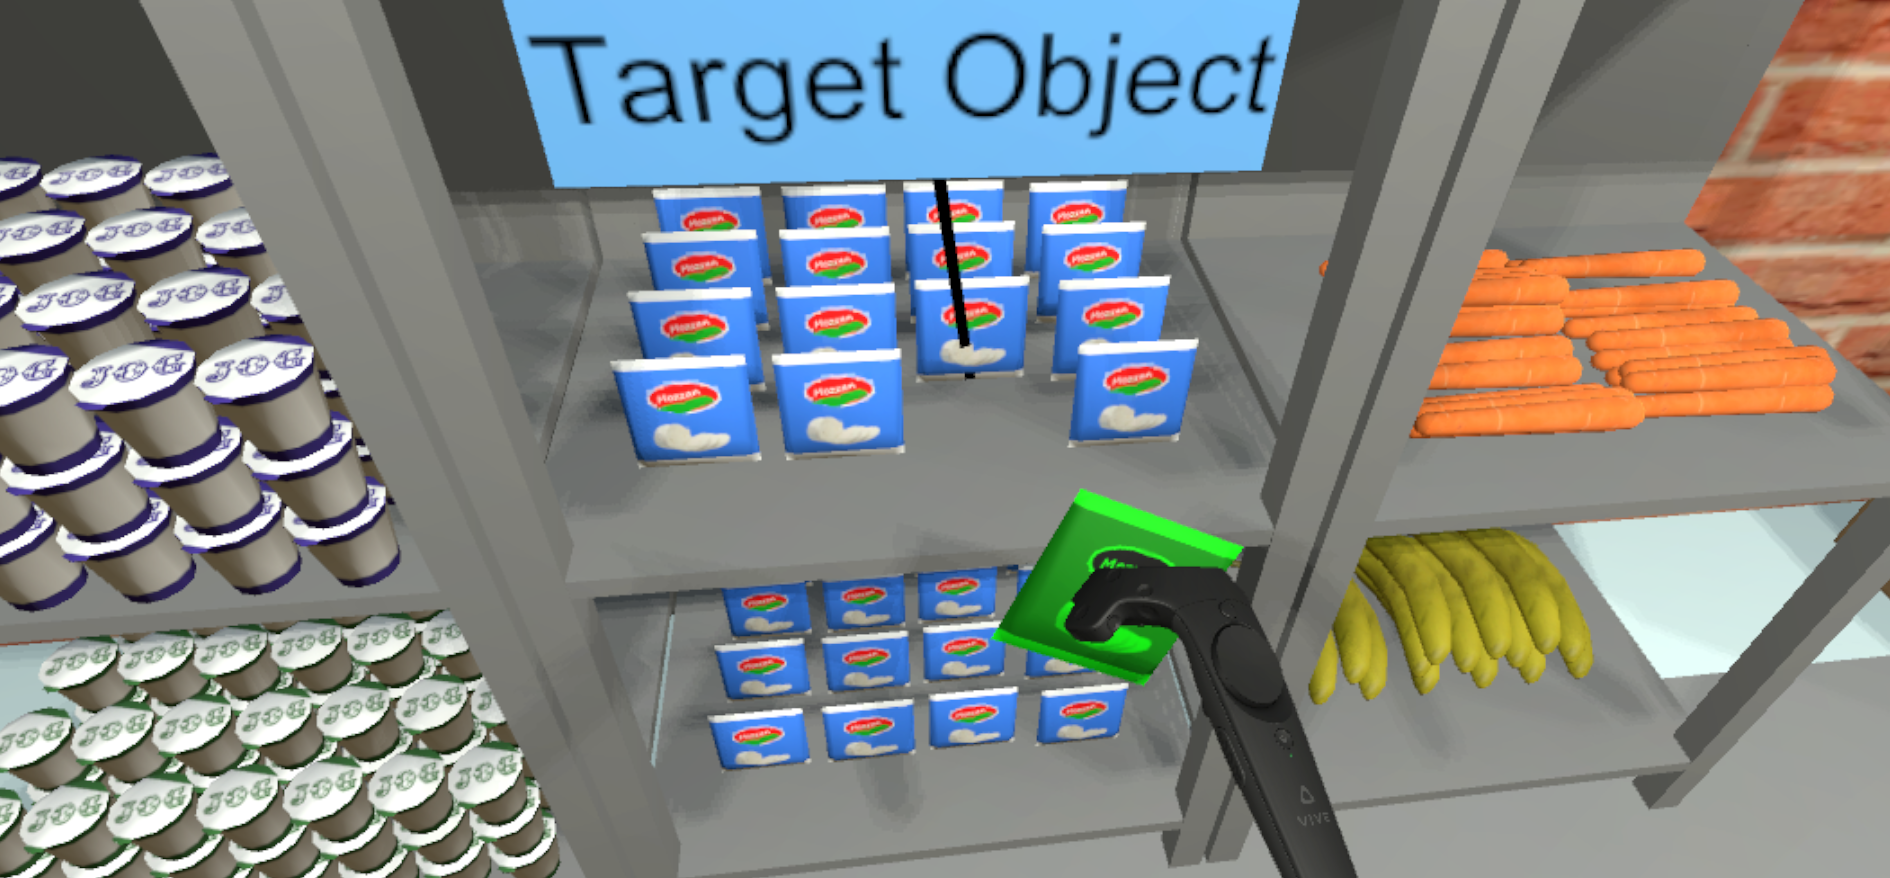
\includegraphics[width=12cm]{Images/TouchGrab.PNG}			
	\caption[Grabbing a virtual object by using \textit{Touch Grab}.]{Grabbing a virtual object by using \textit{Touch Grab}.}
	\label{fig:touchGrab}
\end{figure}

\subsubsection{Close Range: Proximity Grab} \label{sec:ProximityGrab}
\todo[inline, color=red]{Laura}
When it comes to the CR interactions the \textit{Proximity Grab} is by far the most inexact selection. Grabbing and releasing and object are realised by using the trigger of the \textit{HTC Vive}-controller. \textcolor{red}{@Laura: siehe oben?}  \\
The functionality is provided by the script \textit{ProximityGrab.cs}. The basic idea is that the object can be grabbed, whenever the object triggers the \textit{BoxCollider} \cite{website:BoxCollider} placed at the end of the \textit{HTC Vive}-controller. A more detailed description can be found in section \ref{sec:TouchGrab}. In contrast to the \textit{Touch Grab} described in section~\ref{sec:TouchGrab} this \textit{BoxCollider} is bigger than the actual size of the controller. To show the user, which object collides with the controller and can therefore be grabbed, the respective object is coloured green, as shown in figure~\ref{fig:proximityGrab}. The small gap between the actual grabbed object and the controller shows the difference between the interaction method shown in figure~\ref{fig:touchGrab}.

\begin{figure}[H] 
	\center 
	\includegraphics[width=12cm]{Images/ProximityGrab.PNG}			
	\caption[Grabbing a virtual object by using \textit{Proximity Grab}.]{Grabbing a virtual object by using \textit{Proximity Grab}.}
	\label{fig:proximityGrab}
\end{figure}


\subsubsection{Close Range: Wand Grab} \label{sec:WandGrab}
\todo[inline, color=red]{Laura}
In contrast to the interaction method described in \ref{sec:ProximityGrab} this method can be used to grab very tiny objects. Thereby it is not needed that the target object is very isolated from other objects. To give the user such an high grade of accuracy a stick is added to the controller like shown on figure~\ref{fig:wandGrab}. The user can grab an virtual object he touches with the \textit{HTC Vive}-controller by pulling the trigger. To place the object on the target area he simply release the trigger after he moved the object to its destination. \textcolor{red}{@Laura: siehe oben ;)}\\
The implementation can be found in \textit{AllRaycastMethods.cs}. The wand consists of two elements: a ray \cite{website:Ray} and a cube. The cube is only for the visualisation and has a fixed size in all three dimensions. The collision detection, which is necessary for the actual grabbing, is done with the ray. That means that an object can be grabbed if the ray, which has the same dimensions like the cube, touches this specific object. The cube \textcolor{red}{@Laura: vllt 'stick' damit klar ist, dass das am Controller gemeint ist?} will then turn from black to green to show the user that there is an object which can be grabbed.

\begin{figure}[H] 
	\center 
	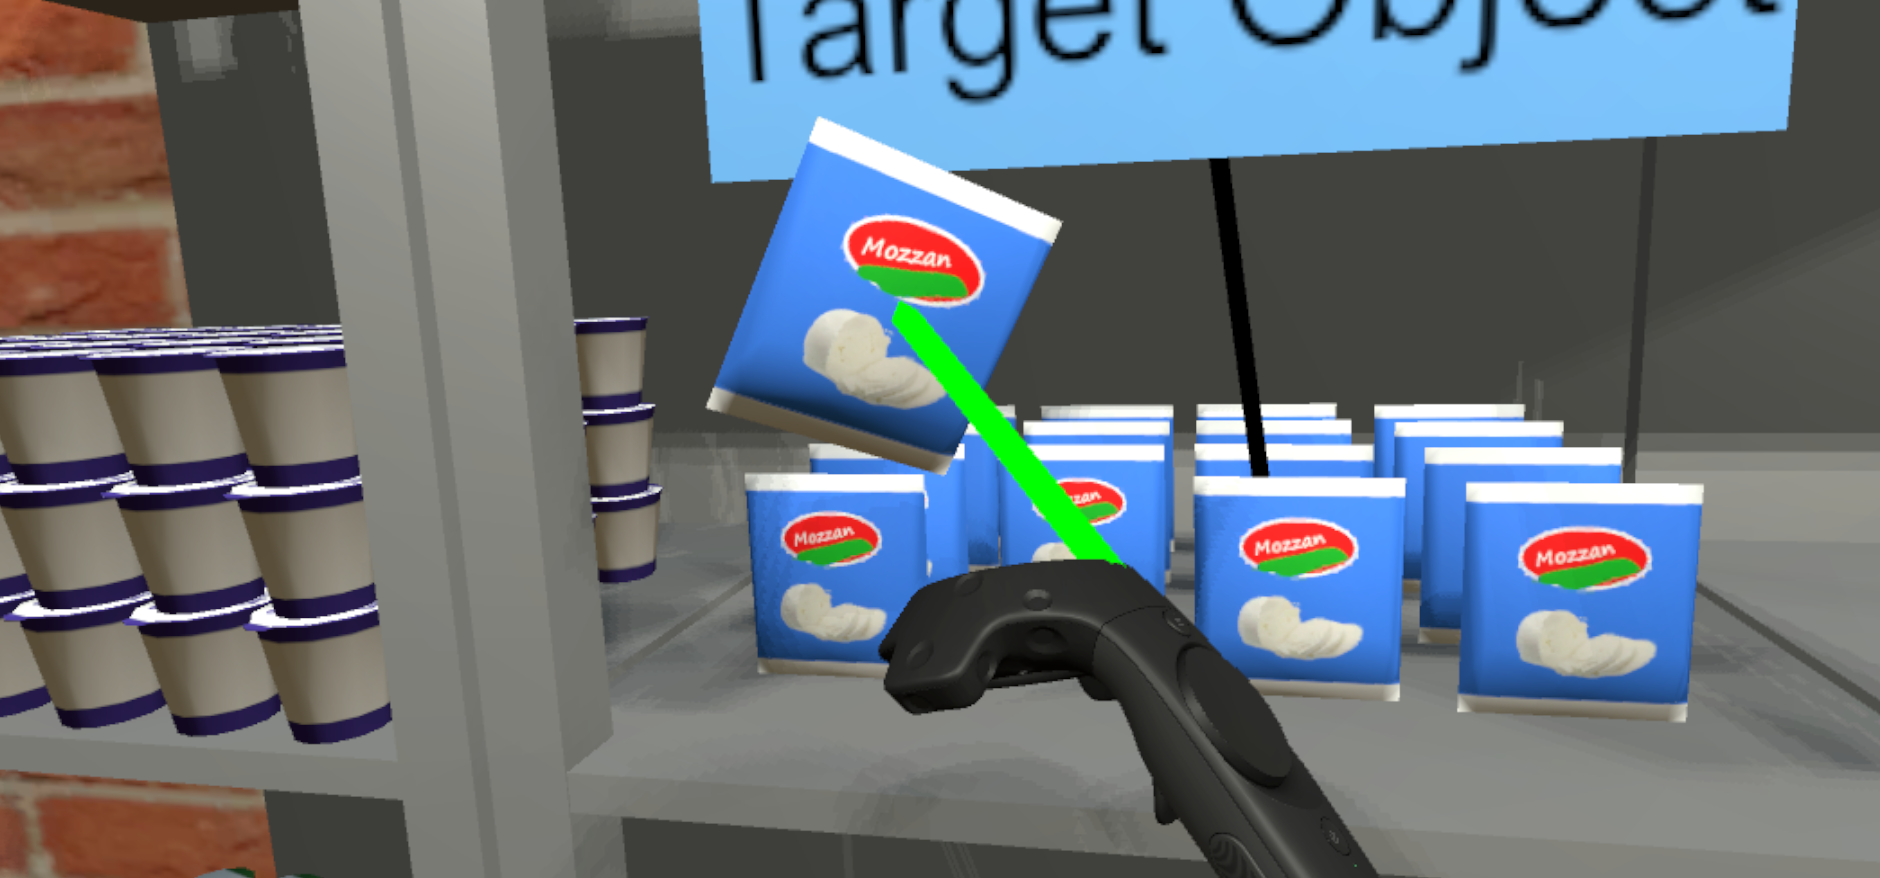
\includegraphics[width=12cm]{Images/WandGrab.PNG}			
	\caption[Grabbing a virtual object by using \textit{Wand Grab}.]{Grabbing a virtual object by using \textit{Wand Grab}.}
	\label{fig:wandGrab}
\end{figure}

\subsubsection{Far Range: Raycast} \label{sec:Raycast}
%\todo[inline, color=yellow]{Laura}
By using the \textit{Raycast} method the user can grab virtual objects which are further away as well as objects in his CR. As shown in figure~\ref{fig:raycast} a ray is coming out of the \textit{HTC Vive}-controller pointing away from the user. At the end of the ray is a small sphere, which turns green, if it collides with an moveable object. Whenever the ray hits an objects, like for example the floor or a product in the supermarket (compare section~\ref{sec:supermarket}), the ray is shortened to the distance between the controller and the respective object. \\
The implementation can be found in the \textit{AllRaycastMethods.cs} script. As already explained in section \ref{sec:WandGrab} a cube and a ray are combined to reach the intended functionality. In contrast to the \textit{Wand Grab}, the ray and the visible cube have no fixed length and there is a sphere added to the end of the cube.

\begin{figure}[H] 
	\center 
	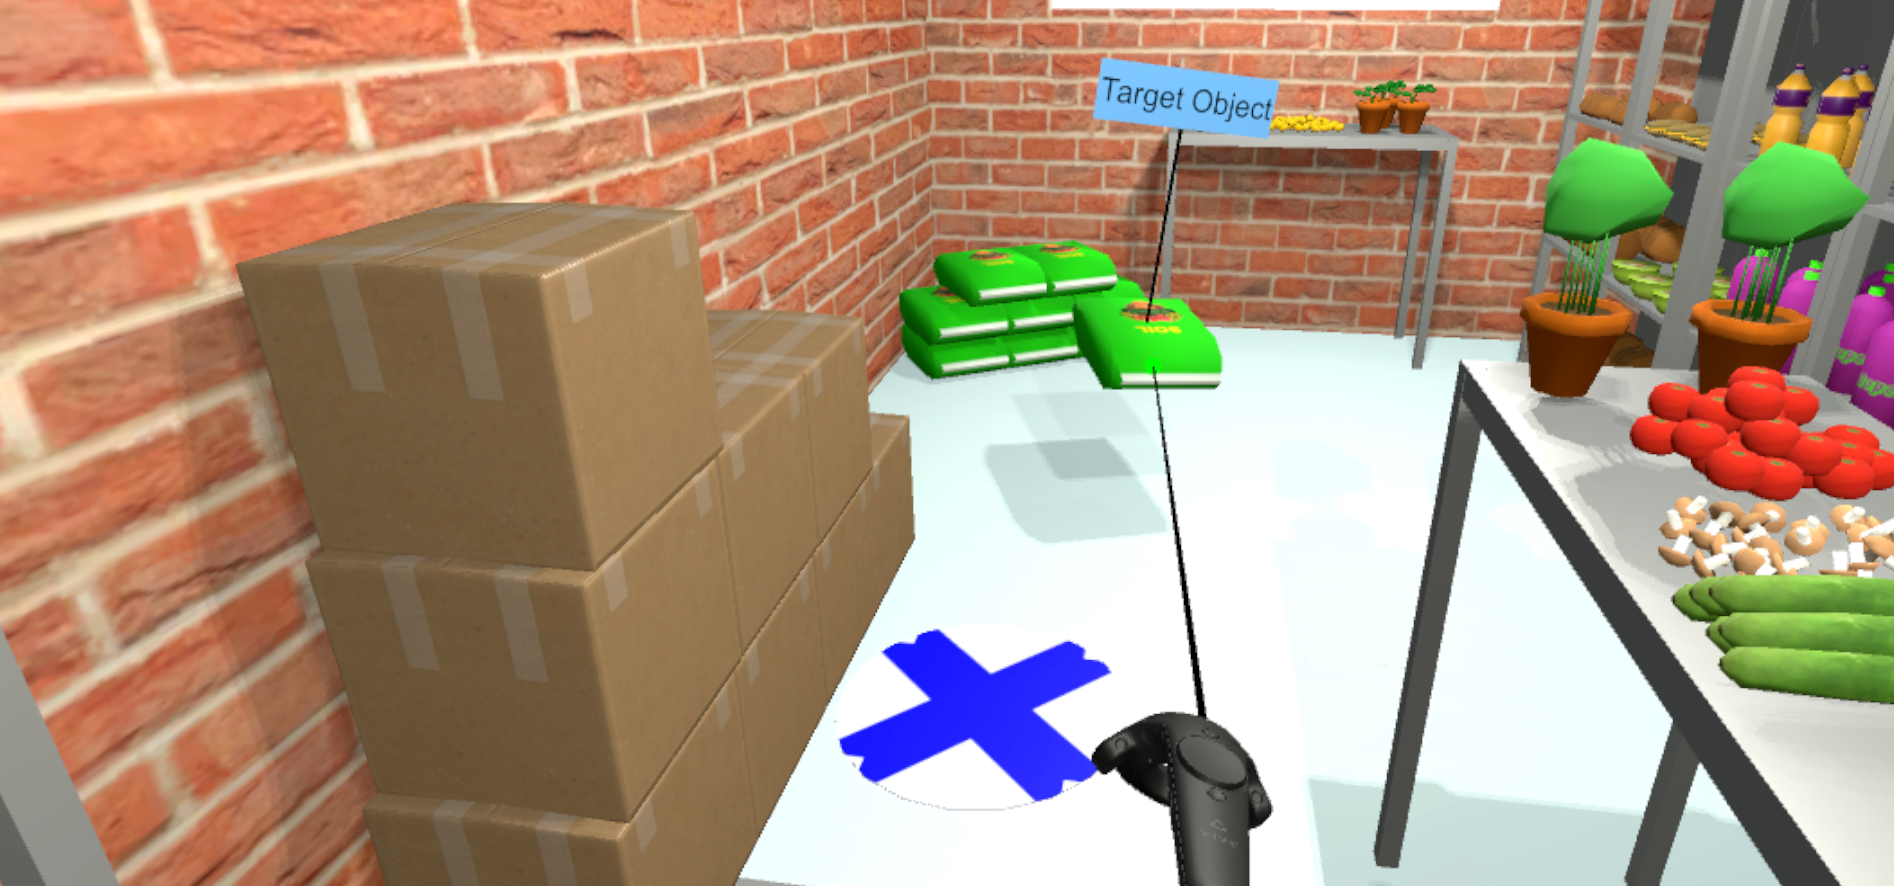
\includegraphics[width=12cm]{Images/Raycast.PNG}			
	\caption[Grabbing a virtual object by using \textit{Raycast}.]{Grabbing a virtual object by using \textit{Raycast}.}
	\label{fig:raycast}
\end{figure}


\subsubsection{Far Range: Extendable Ray} \label{sec:ExtendableRay}
\todo[inline, color=red]{Laura}
The actual ray is build as described in section \ref{sec:Raycast}. The ray \cite{website:Ray} is complemented by a cube with a sphere at the end, to make it visible for the user. \textcolor{red}{@Laura: hast du auch in Raycast beschrieben oder?} In contrast to the normal \textit{Raycast} method the length of the ray is set to a start value of 3 meters. The user can shorten and lengthen the ray by pressing the touchpad of the \textit{HTC Vive}-controller in the lower or rather upper area. This subtracts or adds a constant value to the length of the visible ray. The behaviour of the sphere remains, which turns green, whenever a moveable virtual object is brushed. The \textit{Extendable Ray} is one of the three interactions methods (compare sections~\ref{sec:WandGrab} and~\ref{sec:Raycast}) which are combined in the \textit{AllRaycastMethods.cs} script. This interaction method is shown on figure~\ref{sec:ExtendableRay}.

\begin{figure}[H] 
	\center 
	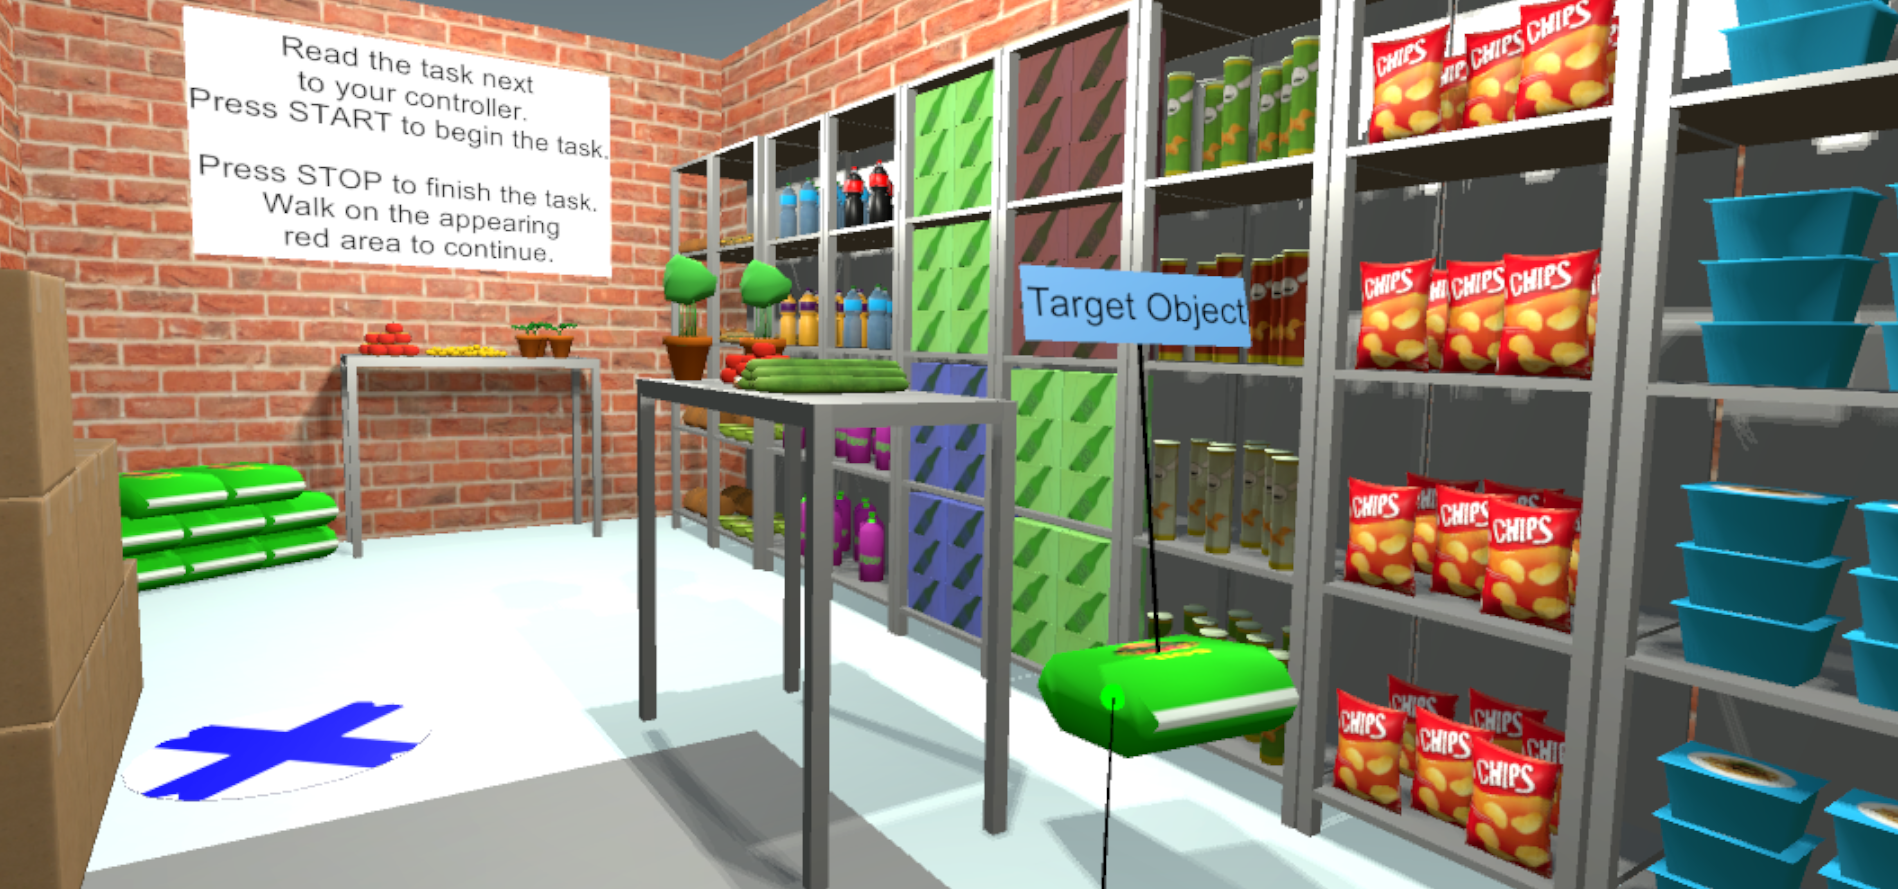
\includegraphics[width=12cm]{Images/ExtendableRay.PNG}			
	\caption[Grabbing a virtual Object by using \textit{Extendable Ray}.]{Grabbing a virtual Object by using \textit{Extendable Ray}.}
	\label{fig:extendableRay}
\end{figure} 


\subsubsection{Far Range: Raycast Head Mounted Display} \label{sec:RaycastHMD}
\todo[inline, color=red]{Laura}
It was planned to realise an interaction method where there is a ray coming out of the HMD which can be used similar to the method described in section~\ref{sec:Raycast}. Due to the low accuracy of this method it did not become a part of the \textit{Interaction Lab}. There was a try to parent \cite{website:SetParent} the position of the HMD to the starting point of the ray. It turned out that the parenting is not successful when it comes to the position and rotation of the HMD. Even this method was effective for adding a ray to the \textit{HTC Vive}-controller, there is a irregular shift when you try to implement it with the HMD. \textcolor{red}{@Laura: ich versteh den satz nicht. welche Methode war effectiv? setParent?} To proof that an easy example (compare source code~\ref{lst:testHMD}) was observed. In this example a simple cube should be rendered at the front of the HMD. In reality this cube was rendered in a position which can be seen as random. 

\lstinputlisting[title=\lstname, caption={Test on the parenting of \textit{HTC Vive}-HMD and an virtual object.}, label=lst:testHMD, language={[Sharp]C}, linerange=1, firstnumber=1]{SourceCode/HMDtest.cs} 

All effort on this method can be found in the script \textit{RaycastingMethodeHMD.cs}.


\subsection{Self-Teaching} \label{sec:selfteaching}
\todo[inline, color=red]{Anna}
To guarantee an easy and smooth introduction to the system, an automatic selfteaching is integrated into the learning room. When the program is started all necessary instructions will be shown next to the controller, like shown in figure~\ref{fig:teaching1}. 

\begin{figure}[H] 
	\center 
	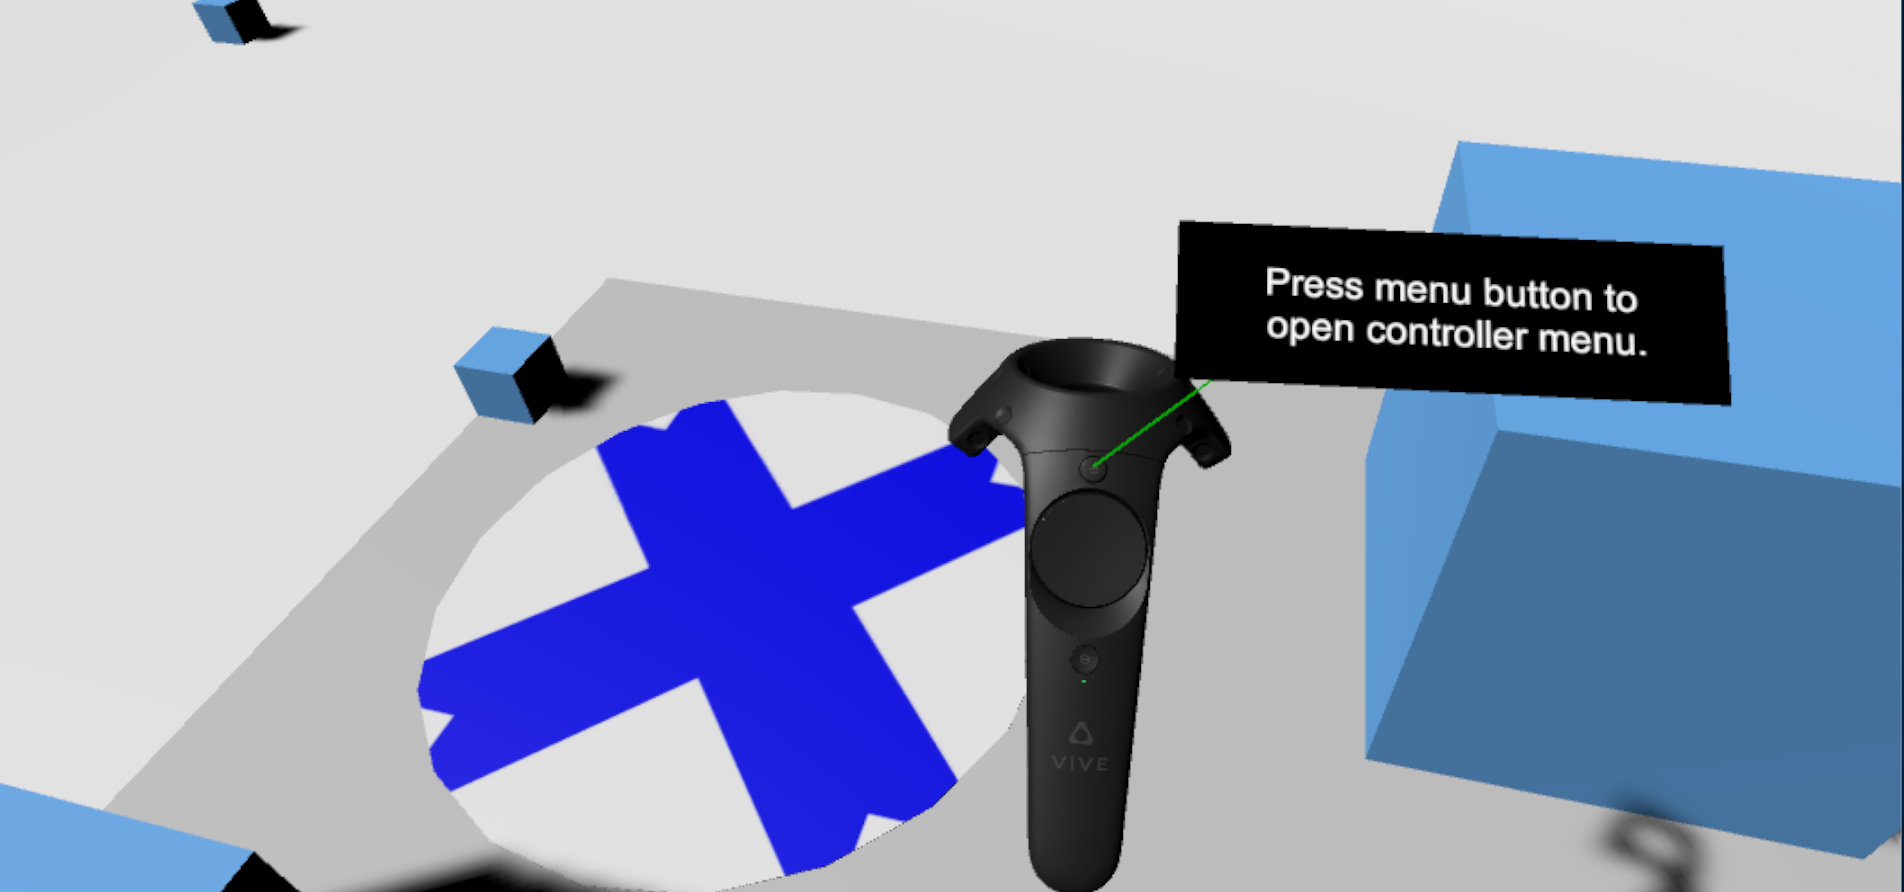
\includegraphics[width=12cm]{Images/teaching.PNG}
	\caption[Start of the Selfteaching.]{Start of the Selfteaching.}
	\label{fig:teaching1}
\end{figure}

This instructions led the user step by step through the system. He will get to know how the interaction methods can be chosen and what settings can be made. Of course the actual grabbing and releasing of an object is taught as well, for every interaction method. 

\begin{figure}[H] 
	\center 
	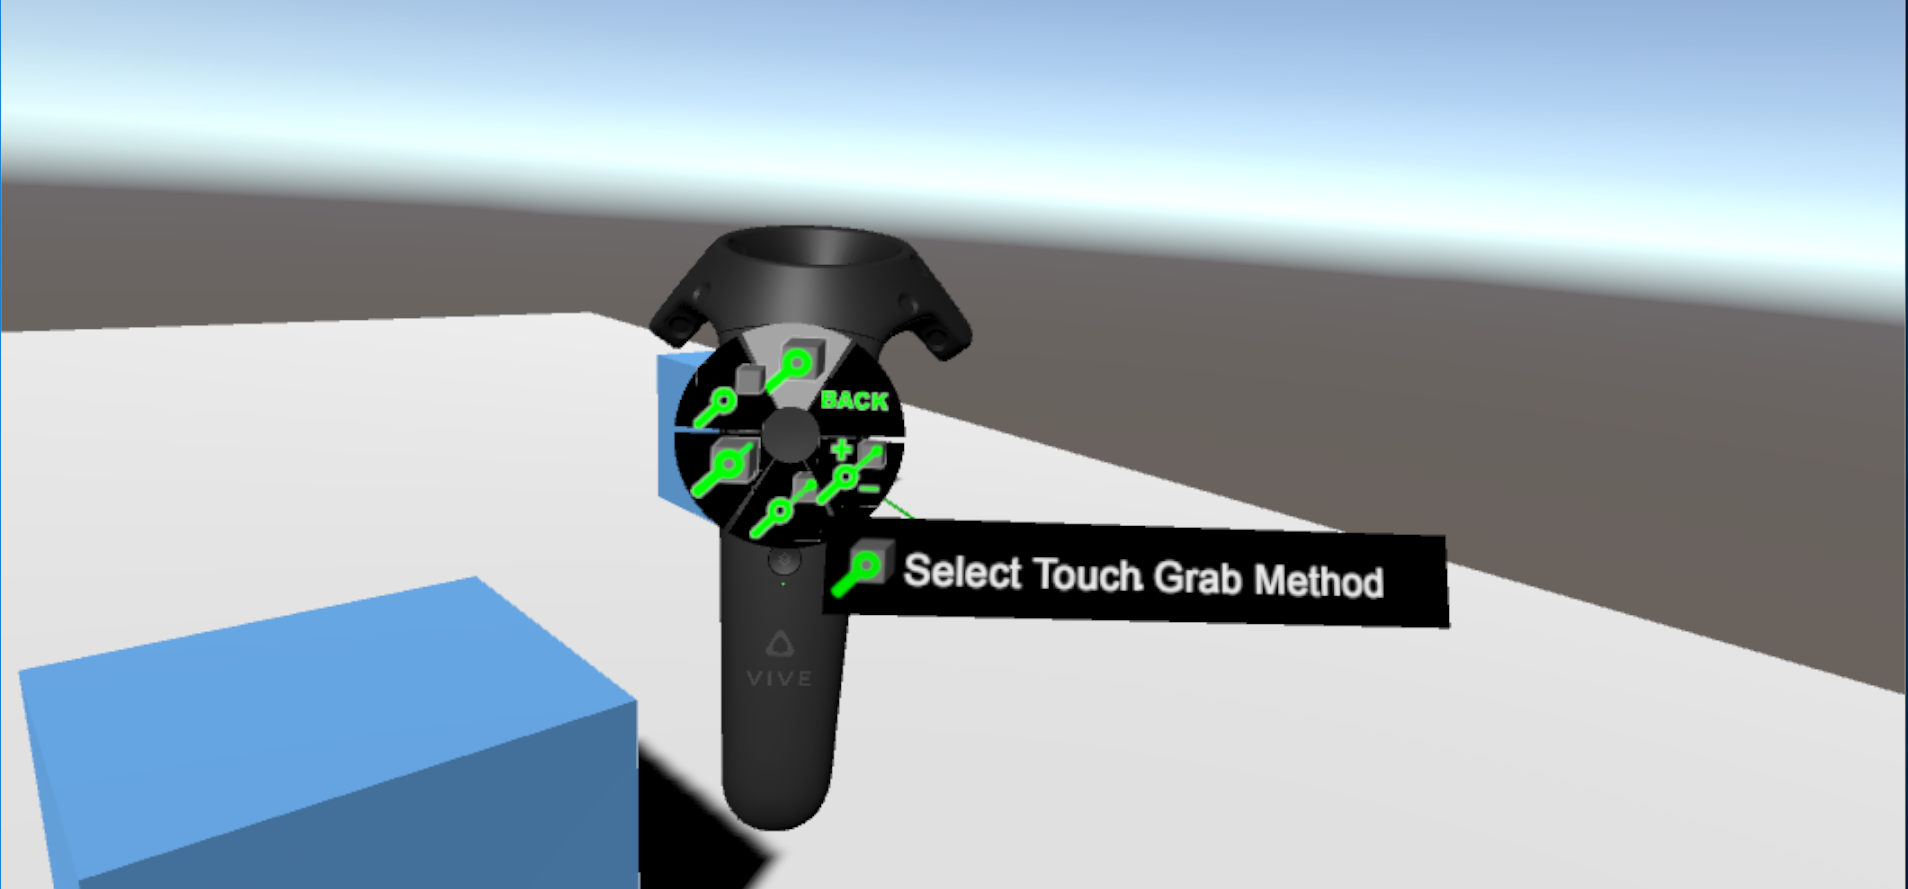
\includegraphics[width=12cm]{Images/teaching2.PNG}
	\caption[Selfteaching recommends to select \textit{Touch Grab} method.]{Selfteaching recommends to select\textit{Touch Grab} method.}
	\label{fig:teaching2}
\end{figure}

The instructions will only be visible in the learning room. The position of the information area changes depending on which button is important for the interaction. \\
In the first grab method, the \textit{Touch Grab} method, two terms will be established, which are important for all tasks. This terms are the labelling of the target object and the target area. Here the user learns how the target object is marked, compare figure \ref{fig:teaching3}, and how the target area reacts to the target object.

\begin{figure}[H] 
	\center 
	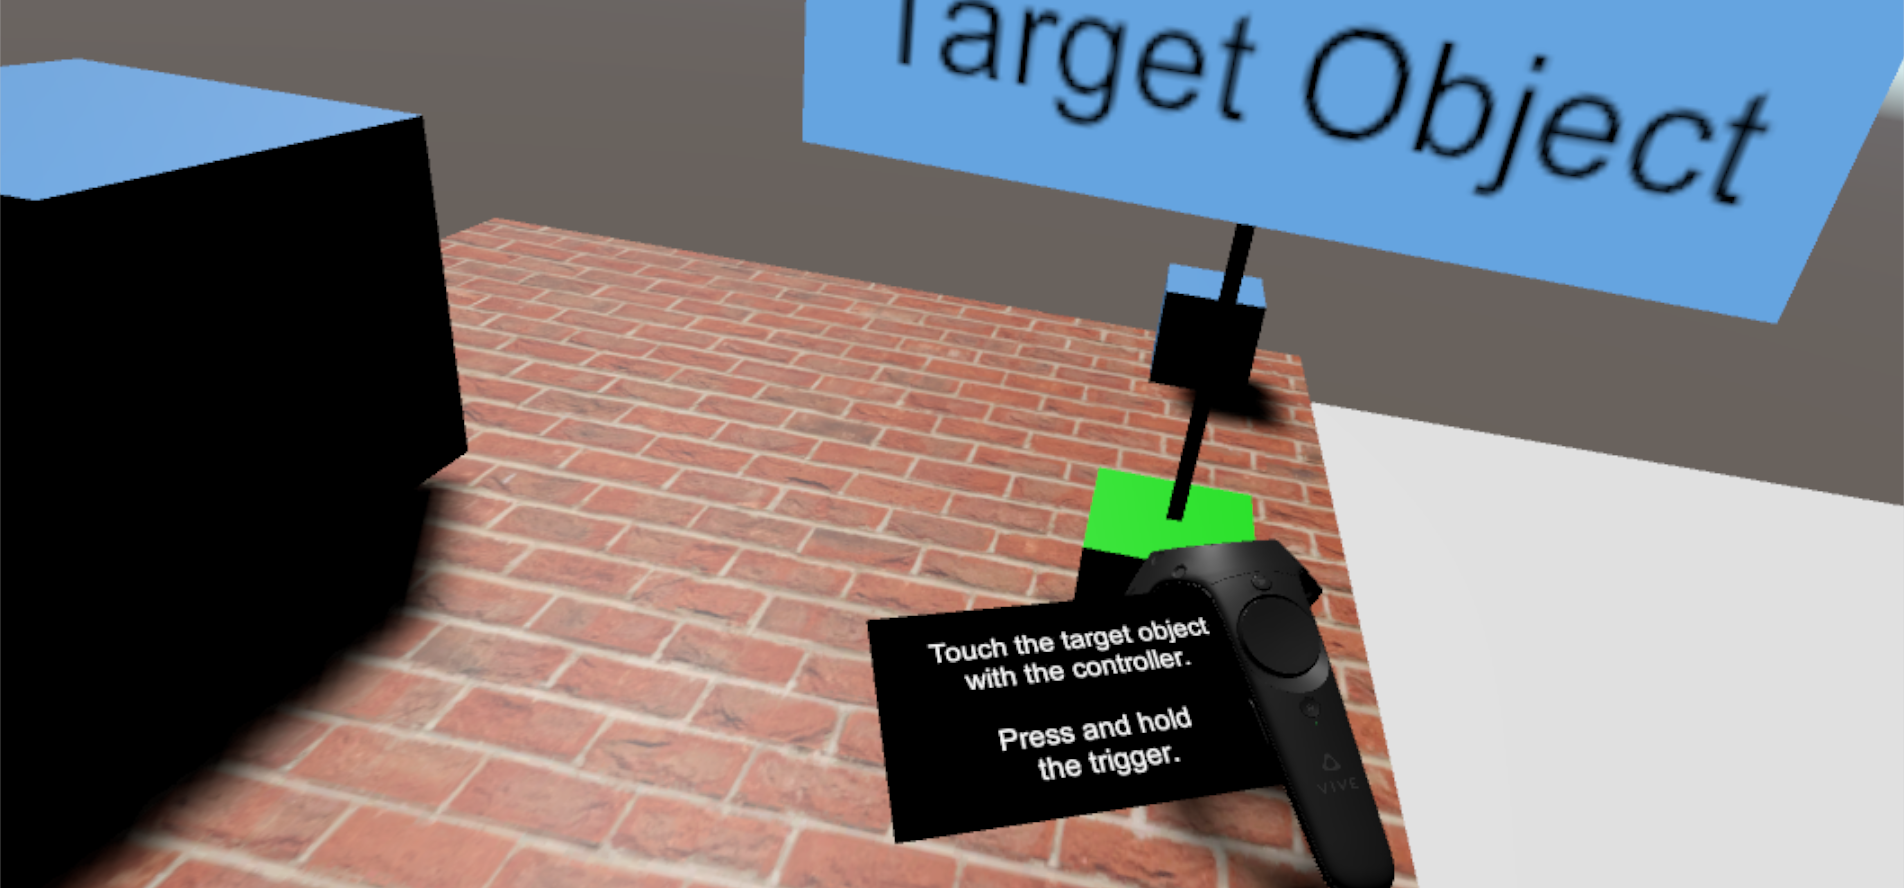
\includegraphics[width=12cm]{Images/teaching3.PNG}
	\caption[Selfteaching with Target Object.]{Selfteaching with Target Object.}
	\label{fig:teaching3}
\end{figure}


\textcolor{red}{@Anna: Vielleicht ist es hier verständlicher wenn du einfach ein Bild von einem Auszug des Files reinpackst? So ist das glaube ich ein wenig kompliziert zum vorstellen. oder was meinst du?}
All instructions and steps of the selfteaching are saved in an external CSV-file. Due to an additional script \textit{WriteMeasureFile.cs} this file will be read line after line and be saved into different lists. In each line are three main information. First there is the text which should be shown in this step. Second is the Button ID, which defines on which button the information should be fixed. Third and last is the height of the information area. This height changes depending on the amount of information. \\
In the \textit{SelfTeaching.cs }script is a counter implemented. This counter controls which line of the file will be displayed. It will be increased or set from different scripts depending on an action. This increasing is still a problem if the user does not follow the selfteaching exactly. For example, if the user grabs an object twice and the selfteaching plans to grab just once, the selfteaching will go on and the user misses instructions. \\
The instruction canvas is also a prefab of the ``VRTK'' plug-in. Here they are called controller tips. This creates a area next to the controller and a line from this area to the selected button of the controller. This area is parented to the controller and moves according to it. Different settings can be changed within the \textit{Unity} editor or by a script.\\
The ``VRTK'' plug-in has also a prefab for object tips. This is also a canvas in which information can be displayed, but this can be fixed on any object you like. With this canvas the target objects are labelled.


\newpage